
\subsection{Machbarkeitsvalidierung}

%    Einfach sieben Sätze was die wichtigsten nicht funktionalen Anforderungen sind.
%    Beispielweise: isolation der Agenten, performante Übertragung.
%    Nicht erklörung der erfolgreichen Umsetzung sondern die definition der Ziele
%    Nicht zu detailiert sonst wird das zu viel.

Für diese Anwendung gab es mehrere sehr zentrale Qualitätsziele.
Diese sind besonders relevant, insofern sie für diese Anwendung ausschlaggebend für die Zweckerfüllung bzw. die Nutzbarkeit sind.
Gleichzeitig ist die Erfüllung dieser für diese Anwendung schwerer als es für klassische Web-Anwendungen der Fall wäre, was nicht zuletzt an den hohen Datenmengen und der Echtzeit-Anforderung liegt.

Um diese Anforderungen zumindest abschätzen zu können, wurde vor der Planung der Anwendung ein technischer Durchstich realisiert, der ermitteln sollte, wie viele Fahrzeuge sich maximal darstellen lassen und welche Framerate dies nach sich ziehen würde.

Dabei wurden Frames durch einen sehr einfachen Generator auf dem Server erstellt und an den Client gesendet, der diese ohne Nachbearbeitung darstellte.
Bei diesem Test ließen sich in etwa 15.000 Fahrzeuge mit 30 Hz bei 1920 px mal 1080 px auf einem System mit einem AMD FX 8320 und einer Nvidia GForce 1060 darstellen bzw. übertragen.

Interessanterweise war zu diesem Zeitpunkt die De-/Serialisierung der Aspekt, der limitierend wirkte.

%    Die hier zu entwickelnde Anwendung soll eine Simulationsplattform sein.
%    Diese soll primär die Grundlagen, also den Betrieb von Agenten, die Definition von Straßensystemen und die Darstellung des aktuellen Zustandes beinhalten.
%
%    Dafür soll ein Client geschaffen werden welcher dem Nutzer erlaubt ein Straßennetz via eines 3D-Editors zu definieren und Agenten durch das Auswählen von Dateien zu definieren.
%    Der Client lädt dann dies an den Server hoch, welcher daraus eine Instanz erzeugt.
%    Diese Instanz besitzt einen gewissen Zustand welchen der Server verwaltet, diesem Zustand übermittelt der Server an den Client welcher diesen darstellt und an den Agenten, welcher aus diesem zusammen mit einen gewissen Zeitschritt einen neuen Zustand erzeugt.
%
%    \begin{figure}[htb]
%        \centering
%        \label{fig:top-down-betrieb}
%        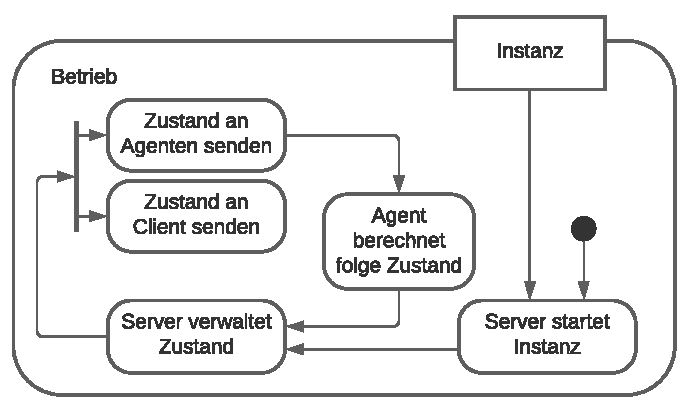
\includegraphics[scale=.65,center]{medien/top-down-betrieb}
%        \caption{Betrieb Ablauf Übersicht}
%        \ownsource
%    \end{figure}
%
%    Mit letzterem ergibt sich dann ein Zyklus, welcher für eine Echtzeit darstellung verwendet werden kann.
%    Durch diese Darstellung kann dann der Nutzer sowohl die Auswirkungen des Straßennetztes als auch das Verhalten des Agenten erkennen.
%
%    Die Anwendung soll als Client-Server Anwendung aufgeteilt werden damit der Server lange laufen kann, mehrer Nutzer auf die gleiche Instanz zugreifen können und Hardware verwendet werden kann welche besonders CPU-Leistungsstark ist.
%    Der Client kann hingegen nach Belieben gestartet werden und mit einer Instanz verbunden werden, dieser Client benötigt, im Gegensatz zu dem Server, eine GPU um die Darstellung des Zustandes zu beschleunigen.
%
%    Der Server ist dabei so zu konstruieren, dass er sich problemlos erweitern lässt, um mehrere Server-Instanzen auf unterschiedlichen Geräten zu nutzen und so die Berechnung zu beschleunigen.
%
%    Hinzu kommt das die gesamte Anwendung so konstruiert werden soll das man sehr leicht weitere Elemente für die Straßenmodellierung hinzufügen kann, so das sich die verschiedensten Szenarien modellieren lassen.

%    Darüber hinaus soll sie leicht erweiterbar sein in den folgendenen drei Aspekten.
%
%    Die Straßen Kacheln. Das
